\chapter{A Computational Implementation of Context Sensitive Distributional Semantics} \label{chap:method}
In the previous chapter, I laid down the theoretical groundwork for a distributional semantic methodology for dynamically establishing perspectives on statistical data about language use.  In this chapter, I'll describe the technical details for building a computational implementation of such a methodology.  The objective of this implementation is to establish a rigorous procedure for generating subspaces of word vectors, based on observations of word co-occurrences in an underlying corpus, the geometries of which are semantically productive in particular contexts.  This will involve three steps:

\begin{enumerate}
\item The selection, processing, and analysis of a large scale textual corpus in order to create a high dimensional base space of co-occurrence statistics;
\item The development of techniques for selecting lower dimensional subspaces based on some sort of contextualising input;
\item The exploration of the geometry of the projected subspaces in search of semantic correlates.
\end{enumerate}

The following three sections will pursue each of these aspects of a technical implementation in turn.  The end result is effectively a mapping from text as raw data to geometry as semiotic generator.  A fourth section will describe an alternative, general interpretation of the statistical data which underwrites my models and additionally offer a brief overview of another distributional semantic methodology, all to be used as a point of comparison in the empirical results which will be discussed in subsequent chapters.

\section{Establishing and Analysing a Large Scale Textual Corpus}
The first step in a corpus based approach to natural language processing is the selection of the data which will provide the basis for our model.  I've picked the English language portion of Wikipedia as my data source, a choice which is in accordance with a good deal of work done in the field.  For instance, \cite{GabrilovichEA2007} and \cite{CollobertEA2008}, to name just a couple, use Wikipedia as their base data for training distributional semantic models designed to perform tasks similar to the ones explored in subsequent chapters, while \cite{BaroniEA2014}, \cite{PenningtonEA2014}, and \cite{GutierrezEA2016} use amalgamated corpora that include Wikipedia as a major component.  Wikipedia provides a very large sample of highly regular language, meaning that we can expect a certain syntactic and semantic consistency as well as language which, if not always overtly literal, is likewise not typically abstruse or periphrasitc.  This should supply a source of linguistic data in which, to revisit the central dogma of the distributional hypothesis, words which occur in a specific syntactic and lexical setting can be expected to be semantically similar.

In the case of my implementations, the November 2014 dump of English language Wikipedia has been used.\footnote{Relatively recent Wikipedia dumps are available at \url{https://dumps.wikimedia.org/}.}  A data cleaning process has been implemented, the first step of which is the chunking of the corpus into individual sentences.  Next parenthetical phrases are removed from each sentence, as these can potentially skew co-occurrence data, and all other punctuation is subsequently removed.  All characters are converted into lowercase to avoid words capitalised at the beginning of sentences, quotations, and other places being considered as unique types.  Finally, the articles \emph{a}, \emph{an}, and \emph{the} are removed as they can distort co-occurrence distance counts.  The cleaned corpus contains nearly 1.1 billion word tokens, consisting of almost 7.5 million unique word types.  The distribution of these types is predictably Zipfian: over 10 million occurrences of the top nine word types are observed, while the least frequent 4.27 million words -- more than half of all types -- only occur once.  The top end of this distribution is populated by conjunctions, prepositions, and pronouns, while the bottom end is characterised by obscure place names, one-off abbreviations, unicode representing non-Latin alphabet spellings, and a good many spelling errors.

As is generally the case with data cleaning, these measures are prone to error: for instance, due to the removal of punctuation, the contraction \emph{we're} will be considered identical to the word \emph{were}.  One of the strengths of the subspace projection technique that my methodology uses is its resilience to noise.  So, for instance, misspellings will be categorised as highly anomalous co-occurrence dimensions and are therefore unlikely to be contextually selected -- or, if they are regularly encountered enough to be contextually significant, there may well be useful information in the co-occurrence profile of such mistakes -- and, at the other end of the spectrum, essentially ubiquitous words are unlikely to provide context specific information, so the ambiguity between \emph{we're} and \emph{were} is unlikely to be drawn into any of the subspaces actually projected by the model.

From the cleaned corpus, a model's vocabulary is defined as the top 200,000 most frequently occurring word types.  This cut-off point is very close to the point where the total number of word tokens included -- that is, occurrences of any word of any type -- by selecting all instances of all vocabulary words equals the total number of word types -- that is, unique word forms -- excluded.  Given the Zipfian distribution of word frequencies as observed throughout the corpus, this means that more than 95\% of the co-occurrence data available from the corpus will be taken into account by the model, while the number of word-vectors used to express this data represents less than 5\% of the potential vocabulary---a fairly efficient way of extrapolating statistics from the corpus.  The selection of this as a cut-off point means that the least frequent words in the vocabulary occur 83 times throughout the corpus.

Having processed the corpus and established the target vocabulary, the next step of this methodology is to build up a based space of co-occurrence statistics.  Here, following the example of the majority distributional semantic work, co-occurrence between a word $w$ and another word $c$ will be considered in terms of the number of other words between $w$ and $c$.  In the case of my methodology, and again in accord with the a great deal of work within the field, a statistic for word $w$ in terms of its co-occurrence with $c$ will be derived from the consideration of all the times that $c$ is observed within $k$ words of $w$, where $k$ is one of the primary model parameters that will be considered in the experiments reported in later chapters of this thesis.  Based on these co-occurrence events, a matrix $M$ is defined, where rows consist of word-vectors, one for each of the 200,000 words in the vocabulary, and columns correspond to terms with which these vocabulary words co-occur.  These column-wise co-occurrence dimensions include the words in the vocabulary as well as many, many words that are not in the vocabulary, to the extent that every word type in the corpus is considered as a candidate for co-occurrence.  A \emph{pointwise mutual information} metric gauging the unexpectedness associated with the co-occurrence of two words is calculated in terms of this equation:

\begin{equation}\label{eq:MI}
M_{w,c} = \log_2 \left(\frac{f_{w,c} \times W}{f_w \times \left(f_c + a\right)} + 1\right)
\end{equation}

Here $f_{w,c}$ represents the total number of times that $c$ is observed as co-occurring in a sentence within $k$ words on either side of $w$, $f_w$ is the independent frequency of occurrences of $w$, and $f_c$ is likewise the overall frequency of $c$ being observed as a co-occurrence term throughout the corpus.  $W$ is the overall occurrence of all words throughout the corpus--and it should be noted that, excluding the term $a$, the ratio in Equation~\ref{eq:MI} is equivalent to the joint probability of $w$ and $c$ co-occurring.  The term $a$ is a skewing constant used to prevent highly specific co-occurrences from dominating the analysis of a word's profile, set for the purposes of the work reported here at 10,000.\footnote{Anecdotally, the first combination of input words analysed during an early stage of the development of this model that didn't use a smoothing constant was the phrase ``musical creativity'', and the very first dimension indicated by the analysis was labelled \emph{gwiggins}---the email handle of one of my supervisors.  Prof. Wiggins's deep connection with music and creativity meant that every instance of \emph{gwiggins} occurring throughout Wikipedia was in the vicinity of both \emph{musical} and \emph{creativity}, and so the dimension was indicated by the combination of these terms, which makes sense, but it was still a bit eerie to have such a personally relevant result generated by a model based on such general data.}  Finally, the entire ratio is skewed by 1 so that all values returned by the logarithm will be greater than 0, with a value of zero therefore indicating that two words have never been observed to co-occur with one another.

This last step of incrementing the ratio of frequencies in order to avoid values tending towards negative infinity in the case of very unlikely co-occurrences is again a departure from standard practice, where, in word counting models, a \emph{positive pointwise mutual information} mechanism involving not skewing the ratio and instead treating any ratio of frequencies less than 1 -- that is, any co-occurrence that is observed less often than the balance of the mean values for all occurrences of $w$ and all co-occurrences with $c$ -- as being equivalent to zero, or no co-occurrence at all \citep[][have considered a more general variable ratio shifting parameter]{LevyEA2014b}.  The motivation for this more typical technique is again to avoid incorporating unnecessary and potentially confounding information into a model, but, again, in the case of my model, the dimensional selection process will tend to ignore such information, and at the same time, as will be seen, data regarding relatively unlikely co-occurrences can sometimes also be quite informative.  Other areas for variation in deriving co-occurrence statistics include the nature of the co-occurrence window itself, where some researchers have taken weighted samples \citep or considered word order, and also the actual representation of tokens within the corpus, where part-of-speech and dependency tagging \citep{PadoEA2007} have been applied to positive effect.  \cite{LapesaEA2014} and \cite{MilajevsEA2016} offer comparative overviews of the effects of parameter variations on the performance of distributional semantic techniques.

The net result of my methodology is a matrix of weighted co-occurrence statistics, where higher values indicate a high number of observations of word $w$ co-occurring with word $c$ relative to the overall independent frequencies of $w$ and $c$.  Values of zero indicate words which have never been observed to co-occur in the corpus, and, as most words never co-occur with one another, the matrix is highly sparse.  The weighting scheme results in a kind of semi-normalisation of the matrix: infrequent words will tend to correspond to more sparse dimensions, but the non-zero values along these dimensions will by the same token tend to be higher due to the lower value of the word's frequency in the denominator.  So far this technique sits comfortably within the scope of existing work in the field.  It is what I propose to do with this base matrix that will begin to distinguish my methodology, and this next step in the process of projecting context sensitive spaces of word-vectors will be discussed in the following section.

\section{Selecting Dimensions from a Sparse Co-Occurrence Matrix}
Context has thus far remained a somewhat abstract concept in this thesis.  In principle, the context in which conceptualisation occurs for a cognitive agent is its environment with all its affordances, linguistic and semantic but also more generally perceptual: in a word, the agent's \emph{umwelt} \citep{VonUexkull1957}.  In the world of physical entanglements, language presents itself with precisely the same open-ended opportunities for action as other modes of cognition---and, in the case of language, the action afforded is meaning making.  In practice, however, for the purposes of my methodology, context will be defined lexically, as a word or set of words which are fed to a model, analysed in terms of their co-occurrence profiles, and then used to generate a subspace of conceptually relevant co-occurrence dimensions.  The intuition behind this approach is the idea that there should be a set of words which collectively selects a set of dimensions that are conceptually relevant to some conceptual context, and the geometry of the word-vectors of my model vocabulary as projected into the subspace delineated by this set of dimensions should reveal the semantics of this context.

So, notwithstanding interesting work on multi-modal approaches to distributional semantics from, for instance, \cite{HillEA2014} and \cite{BruniEA2014}, with regard to the present technical description, I will treat \emph{context} as meaning some set of words $T$ which have been selected for the purpose of performing some type of semantic evaluation and act as input to a context sensitive distributional semantic model.  The exact mechanisms for specifying $T$ will be discussed in subsequent chapters with regard to each of the individual experiments to be performed using my methodology; for now, I offer a general outline.  Each component of $T$ points to a word-vector in the matrix $M$ described in the previous section, and the collection of word-vectors corresponding to $T$ serve as the basis for an analysis leading to the projection of a context specific subspace $S$.  I propose three basic techniques for generating these projections, with the model parameter $d$ indicating the specified dimensionality of the subspace to be selected:

\begin{description}
\item[Joint] A subspace of $d$ dimensions with non-zero values for all elements of $T$ and the highest mean PMI values across all elements of $T$ is selected;
\item[Indy] The top $d/|T|$, where $|T|$ is the cardinality of $T$, dimensions are selected for each element of $T$ regardless of their values for other elements of $T$, and then these dimensions are combined to form a subspace with dimensionality $d$;
\item[Zipped] The top dimensions for each element of $T$ are selected as in the \textsc{indy} technique, with the caveat that all selected dimensions must have non-zero values for all elements of $T$ and no dimension is selected more than once.
\end{description}

These techniques are used for the purpose of analysis, and, once this analysis has been performed, the subset of dimensions returned is used to project the entire model vocabulary onto a $d$ dimensional subspace.  The \textsc{joint} technique requires the greatest finesse, as there is an element of cross-dimensional comparison at play.  As such, for the purposes of this technique, the word-vectors selected by $T$ are merged, dimensions with non-zero values for any of the word-vectors are discarded, and the resulting truncated word-vectors, each consisting of an equal number of non-zero dimensions, are normalised.  This ensures that certain elements of $T$ won't dominate the analysis: because the frequency of each word in $T$ applies a deflationary pressure on the PMI values associated with the corresponding word-vectors, very infrequent words would be liable to dominate the analysis with the associated high PMI values in their profile.  This effect is illustrated in Table~\ref{tab:norms}, where PMI values for the top dimensions selected using the \textsc{joint} type subspace by the words \emph{guitar}, which at 88,285 occurrences is ranked 1541 in frequency, are compared with those for the word \emph{dulcimer}, which occurs 516 times and is ranked 62,313 (the base model here was constructed using a 5x5 word co-occurrence window).  Among the dimensions with non-zero values for both words, normalisation brings the respective co-occurrence profiles more in line with one another, facilitating the selection of a subspace which is jointly characteristic of the input terms.

\begin{table}
\centering
\begin{tabular}{llrrlrrlrr}
\hline
& \multicolumn{3}{c}{\emph{guitar}} & \multicolumn{3}{c}{\emph{dulcimer}} \\
& dimension & PMI & normalised & dimension & PMI & normalised \\
\hline
\parbox[t]{2mm}{\multirow{5}{*}{\rotatebox[origin=c]{90}{\textsc{high}}}} & \emph{mandolin} & 8.30964 & 0.10719 & \multicolumn{1}{|l}{\emph{hammered}} & 13.97749 & 0.09354 \\
& \emph{bass} & 8.08501 & 0.10429 & \multicolumn{1}{|l}{\emph{dulcimer}} & 12.73992 & 0.08526 \\
& \emph{12-string} & 8.07679 & 0.10418 & \multicolumn{1}{|l}{\emph{autoharp}} & 11.50399 & 0.07699 \\
& \emph{acoustic} & 7.99076 & 0.10308 & \multicolumn{1}{|l}{\emph{appalachian}} & 11.23224 & 0.07517 \\
& \emph{banjo} & 7.96400 & 0.10057 & \multicolumn{1}{|l}{\emph{zither}} & 10.98302 & 0.07350 \\
\hline
\parbox[t]{2mm}{\multirow{5}{*}{\rotatebox[origin=c]{90}{\textsc{low}}}} & \emph{\emph{attacked}} & 0.05222 & 0.00067 & \multicolumn{1}{|l}{\emph{him}} & 0.25698 & 0.00172 \\
& \emph{report} & 0.04768 & 0.00062 & \multicolumn{1}{|l}{\emph{school}} & 0.25340 & 0.00170 \\
& \emph{country} & 0.04418 & 0.00057 & \multicolumn{1}{|l}{\emph{would}} & 0.23825 & 0.00159 \\
& \emph{champions} & 0.02644 & 0.00034 & \multicolumn{1}{|l}{\emph{into}} & 0.21336 & 0.00143 \\
& \emph{regions} & 0.02538 & 0.00033 & \multicolumn{1}{|l}{\emph{there}} & 0.21320 & 0.00143 \\
\hline
\end{tabular}
\caption{The top five and bottom five dimensions by PMI value for the words \emph{guitar} and \emph{dulcimer}, out of all the dimensions with non-zero values for both words, with scores tabulated independently for each word.}
\label{tab:norms}
\end{table}

In the cases of the \textsc{indy} and \textsc{zipped} techniques, the selectional process is more straightforward, since mean values between word-vectors are not being considered.  Where the \textsc{joint} technique is intended to discover subspaces that represent an amalgamation of the input terms, the \textsc{indy} technique is expected to produce a subspace where individual conceptual characteristics of the input terms, captured as collections of co-occurrence dimensions, are distilled into distinct geometric regions.  The \textsc{zipped} technique might be seen as something of a hybrid of the \textsc{joint} and \textsc{indy} techniques, since it used the \textsc{indy} approach to make selections from the intermediary space of non-zero dimensions available to the \textsc{joint} technique.  In each instance, these techniques are formulated to return a set of dimensions which, with varying degrees of cohesion, delineate a space that is in some sense salient to the contextual terms $T$ serving as the basis for the analysis.  In all cases, these techniques are used for the purpose of analysis, and, once this analysis has been performed, the subset of dimensions returned is used to project the entire model vocabulary onto a $d$ dimensional subspace.

In order to offer a sense of what's happening with these dimensions selection techniques, a preliminary and intuitively motivated case study of dimension selection is outlined in Table~\ref{tab:dims}, again derived from a base space generated through observations made within a 5x5 word co-occurrence window over the course of the corpus.  The top dimensions selected by each technique are presented for two different three term sets of input words: \emph{lion}, \emph{tiger}, and \emph{bear}, on the one hand, which are taken to represent in their union exemplars of wild animals, and on the other hand \emph{dog}, \emph{hamster}, and \emph{goldfish}, which are prototypical pets.  The dimensions selected by the \textsc{joint} technique in response to the \textsc{wild animal} type input include the names of other wild animals, as well as \emph{paw}, a component of many wild animals, \emph{mauled}, an activity performed by wild animals, and, interestingly, \emph{mascot}, presumably because many sports teams take these types of animals as their mascot: while this connection may not be immediately intuitive, it seems likely that this word would probably select for other wild animals in terms of its co-occurrence profile.  The dimensions returned by the \textsc{indy} technique, on the other hand, are, as expected, more independently characteristic of each of the input terms, with culturally referential words like \emph{cowardly} (presumably from many mentions of the Cowardly Lion character from \emph{The Wizard of Oz}) and \emph{crouching} (indicating the popular Chinese movie \emph{Crouching Tiger, Hidden Dragon}), as well as other species-specific terms such as \emph{sumatran} and \emph{grizzly}.  Notably, the term \emph{stearns} pops up here, certainly because of prolific references on Wikipedia to the defunct investment bank Bear Stearns, illustrating ways in which the \textsc{indy} technique might allow for dimensions indicative of underlying polysemy.

\begin{table}
\centering
\begin{tabular}{llllll}
\hline
\multicolumn{3}{c}{\emph{lion, tiger, bear}} & \multicolumn{3}{c}{\emph{dog, hamster, goldfish}} \\
\textsc{joint} & \textsc{indy} & \textsc{zipped} & \textsc{joint} & \textsc{indy} & \textsc{zipped} \\
\hline
leopard & cowardly & cowardly & \multicolumn{1}{|l}{pet} & sled & dog \\
cub & crouching & sumatran & \multicolumn{1}{|l}{hamster} & hamster & hamster \\
hyena & localities & grizzly & \multicolumn{1}{|l}{goldfish} & goldfish & goldfish \\
sloth & rampant & tamer & \multicolumn{1}{|l}{hamsters} & hound & pet \\
lion & sumatran & leopard & \multicolumn{1}{|l}{domesticated} & djungarian & hamsters \\
mascot & grizzly & teddy & \multicolumn{1}{|l}{breed} & koi & fancy \\
paw & wardrobe & tamarin & \multicolumn{1}{|l}{fancy} & nassariidae & breed \\
tiger & leopard & tiger & \multicolumn{1}{|l}{pets} & ovary & siberian \\
rhinoceros & stearns & polar & \multicolumn{1}{|l}{bred} & carp & domesticated \\
mauled & teddy & passant & \multicolumn{1}{|l}{robotic} & ednas & cat \\
\hline
\end{tabular}
\caption{The top 10 dimensions returned using three different dimensional selection techniques, featuring one set of input terms collectively referring to wild animals and another set collectively referring to pets.}
\label{tab:dims}
\end{table}

Similar effects are observed in response to the \textsc{pet} type input.  The word \emph{pet}, two of the three input terms themselves, and the names of other types of pets appear in the output from the \textsc{joint} technique, as well as descriptive terms such as \emph{domesticated}, \emph{breed}, and, amusingly but not irrelevantly, \emph{robotic}, presumably because of the phenomenon of robotic pets, which has its own page on Wikipedia.  The \textsc{indy} technique, on the other hand, returns some very term specific dimensions, again indicating a degree of ambiguity, such as \emph{djungarian} (a breed of hamster popular as a house pet), \emph{nassariidae} (in fact a species of snail, known colloquial as the \emph{dog whelk}), and \emph{ednas} (Edna's Goldfish was a short-lived American punk rock band).  In the cases of both \textsc{pets} and \textsc{wild animals}, the dimensions returned by the \textsc{zipped} technique represent something of an intermediary between the two other techniques, tending to include some of the terms generated using the \textsc{joint} technique but also some more word-specific terms.  The actual geometry of these spaces will be discussed generally in the next section, and will be explored in detail in relation to specific semantic applications in subsequent chapters.

A very broadly similar approach to distributional semantics has been proposed by \cite{PolajnarEA2014}, who describe a \emph{context selection} methodology for generating word-vectors, involving building a base space of co-occurrence statistics and then transforming this space by preserving only the highest values for each word-vector up to some parametrically determined cut-off point, setting all other values to zero.  Setting the cut-off point relatively stringently -- generating a base space of more sparse word-vectors, followed by various dimension reduction techniques -- led to improvements in results on both word similarity and compositionality tests.  This suggests that allowing word-vectors to shed some of their more obscure co-occurrence statistics leads to a more sharply defined semantic space, and indeed there may be an element of disambiguation at play here, as well, with vectors dropping some of the numbers associated with less frequent alternate word senses.

In the end, though, the method described by \citeauthor{PolajnarEA2014} results in a space which, while the information contained in the representation of a particular word is to a certain extent focused on the most typical co-occurrence features of that word, is still fundamentally general and static.  To the extent that any contextualisation takes place here, it happens \emph{a priori} and is cemented into a fixed spatial relationship between word-vectors.  This is anathema to the theoretically grounding of my methodology, which holds that conceptual relationships arise situationally, and that semantic representations should therefore likewise come about in an \emph{ad hoc} way.  The novelty, and, I will argue, the power of my approach lies in its capacity to generate bespoke subspaces in reaction to semantic input as it emerges, and the expectation is that these subspaces will have a likewise context specific geometry which can be explored in order to discover situationally significant relationships between the projected semantic representations.  The next section will begin to examine how these geometries might look.

\section{Exploring the Geometry of a Context Specific Subspace}
Before delving into the question of the types of geometries my method might be expected to generate, I would like to raise a point regarding the typical application of the term \emph{geometry} to vector space models of distributional semantics in the first place.  \cite{Widdows2004} makes an enthusiastic and compelling case for the representational power of geometry, while \cite{Clark2015} has pointed out that treating words as geometric features endows lexical representations with ``significant internal structure'' (p. 509) which can be applied towards modelling the meaning making compositionality of language.  \cite{BaroniEA2014b} go so far as to suggest that their distributional semantic model effectively instantiates the abstract principles of Frege's work on the logic of natural languages \citep{Dummett1981} in a geometric mode.  These are powerful points touching on the essence of semiotics, and the idea that representations that map from data to interpretable features in a space are core to my own methodology.

The point I would like to make now, though, is that there are different degrees of geometry that can be in principle accessed in a vector space of real valued dimensions.  The great majority of approaches surveyed here, taken to be representative of the historical and ongoing trend in the field, present models consisting of spaces of normalised word-vectors, in which there is a monotonic correlation between the distance and the angle between two word-vectors.  In the case of models built using a principal component analysis, this is because when eigenvectors are used as dimensions of maximal variance, there is no meaningful interpretation of sign along these dimensions; in fact, mean values along a dimension will tend towards zero and the signs of values along any dimension discovered through a singular value decomposition can be reversed without any degradation of the information available from the analysis \citep{AbdiEA2010}.  So, while Euclidean distance is strictly meaningful in such a dimensional reduction, there is no sense of a centre of the space other than the centre of gravity of the data as projected onto the selected number of eigenvectors, and cosine similarity is in practice the measure used to determine the similarity between two word-vectors.  And in the case of models built using neural networks, there is no meaningful interpretation of dimensions to begin with, so the resulting space is a \emph{de facto} hypersphere of word vectors that are only relative in terms of their relationship to one another, not their relationship to any objective features of the space.

In the case of my methodology, however, precise values along dimensions, and, correspondingly, overall Euclidean distances are significant: because base dimensions are preserved in the spaces projected through any of the dimension selection techniques described above, the actual position of word-vectors in space, not just their relative situations on the surface of a normal hypersphere, are significant, with a number of potentially desirable effects.  The first effect to note is that in my subspaces distance from the origin is expected to be a meaningful feature.  In a subspace of contextually selected dimensions, word-vectors with strong co-occurrence tendencies for that set of dimensions should have high PMI values across all dimensions, and so a relatively high norm of a word-vector is anticipated to correspond to semantic saliency within that context.

The second effect is that there is a notion of centre and periphery in my subspaces.  Since all values are positive, a word-vector with high scores across all or most dimensions in a subspace will be far from the origin and in the central region of the space.  A further consequence of the positivity of these subspaces is that word-vectors with mainly low or null PMI values will be far from the centre, so in the end two word-vectors may be both close to the centre of a subspace, or at the periphery of a subspace but close to one another, or at the periphery and far from each other, at two different edges of the positively valued space, and each of these situations can be predicted to have a particular semantic interpretation.  The third effect, which follows from the first two points, is that a subspace can be characterised in terms of a set of key points based on an analysis of the collective profiles of the dimensions delineating the subspace, by which I mean some straightforward assessments of the statistical distribution of each dimension involved.

\begin{figure}%[!ht]
  \centering%\vspace*{-2cm}
  \begin{subfigure}[]{0.45\textwidth}
  \centering
  \small
  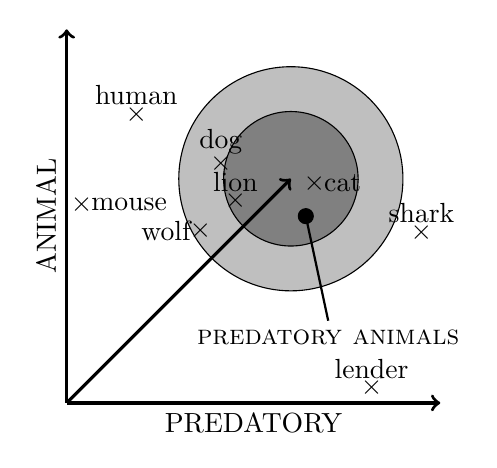
\begin{tikzpicture}
%    \begin{axis}[disabledatascaling,scale=1.75,axis equal,hide axis]
    \begin{axis}[disabledatascaling,scale=1,axis equal,hide axis]
      \draw [fill = lightgray,fill opacity = 1.00] (3,3) circle [radius = 1.5];
      \draw [fill = gray,fill opacity = 1.00] (3,3) circle [radius = 0.9];
      \node at (4.7477,2.2786) [above] {shark};
      \node at (4.7477,2.2786) {$\times$};
      \node at (2.0626,3.2008) [above] {dog};
      \node at (2.0626,3.2008) {$\times$};
      \node at (3.3145,2.9414) [right] {cat};
      \node at (3.3145,2.9414) {$\times$};
      \node at (4.0803,0.2) [above] {lender};
      \node at (4.0803,0.2) {$\times$};
      \node at (2.258,2.7022) [above] {lion};
      \node at (2.258,2.7022) {$\times$};
%      \draw [dotted] (3,3)--(2.258,2.7022) node [midway,above] {$a$};
      \node at (1.7883,2.3021) [left] {wolf};
      \node at (1.7883,2.3021) {$\times$};
      \node at (0.9311,3.8643) [above] {human};
      \node at (0.9311,3.8643) {$\times$};
%      \draw [dotted] (3,3)--(0.9311,3.8643) node [midway,above] {$b$};
      \node at (0.2,2.6516) [right] {mouse};
      \node at (0.2,2.6516) {$\times$};
      
      \addplot [->,very thick] coordinates{
      	(0,0)
        (3,3)
      };
      \node at (3.5,1.1) [below] {\textsc{predatory animals}};
      \addplot [thick] coordinates{
        (3.5,1.1)
        (3.2,2.5)
      };
      \draw [fill=black] (3.2,2.5) circle [radius = 0.1];
%      \addplot [->,dashed] coordinates{
%        (3,3)
%        (3.7,2.4343)
%      } node [midway,below] {$r_1$};
%      \addplot [->,dashed] coordinates{
%        (3,3)
%        (2.1,4.2)
%      } node [midway,above] {$r_2$};
      \addplot [->,very thick] coordinates{
        (0,0)
        (0,5)
      } node [midway,above,sloped] {ANIMAL};
      \addplot [->,very thick] coordinates{
        (0,0)
        (5,0)
      } node [midway,below] {PREDATORY};
    \end{axis}
  \end{tikzpicture}
  \caption{Word-vectors measured by proximity to a central point.}\label{fig:geo1-dist}
  \end{subfigure}
  \hspace*{0.05\textwidth}
  \begin{subfigure}[]{0.45\textwidth}
  \centering
  \small
  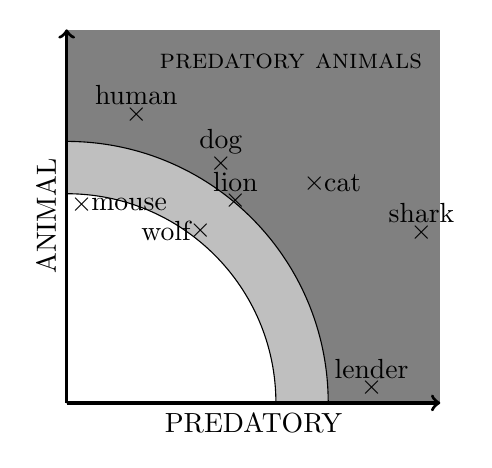
\begin{tikzpicture}
    \begin{axis}[disabledatascaling,scale=1,axis equal,hide axis]
      \draw [white,fill = gray,fill opacity = 1.00] (0,0) rectangle (5,5);
      \draw [fill = lightgray,fill opacity = 1.00] (0,0) -- (3.5,0) arc (0:90:3.5);
      \draw [fill = white,fill opacity = 1.00] (0,0) -- (2.8,0) arc (0:90:2.8);
      \node at (4.7477,2.2786) [above] {shark};
      \node at (4.7477,2.2786) {$\times$};
      \node at (2.0626,3.2008) [above] {dog};
      \node at (2.0626,3.2008) {$\times$};
      \node at (3.3145,2.9414) [right] {cat};
      \node at (3.3145,2.9414) {$\times$};
      \node at (4.0803,0.2) [above] {lender};
      \node at (4.0803,0.2) {$\times$};
      \node at (2.258,2.7022) [above] {lion};
      \node at (2.258,2.7022) {$\times$};
%      \draw [dotted] (0,0)--(2.258,2.7022) node [midway,above] {$a$};
      \node at (1.7883,2.3021) [left] {wolf};
      \node at (1.7883,2.3021) {$\times$};
      \node at (0.9311,3.8643) [above] {human};
      \node at (0.9311,3.8643) {$\times$};
%      \draw [dotted] (0,0)--(0.9311,3.8643) node [midway,above] {$b$};
      \node at (0.2,2.6516) [right] {mouse};
      \node at (0.2,2.6516) {$\times$};
      
      \node at (3,4.8) [below] {\textsc{predatory animals}};
%      \addplot [->,dashed] coordinates{
%        (0,0)
%        (2.8723,2.0)
%      } node [midway,below] {$r_1$};
%      \addplot [->,dashed] coordinates{
%        (0,0)
%        (2.6153,1.0)
%      } node [midway,above] {$r_2$};
      \addplot [->,very thick] coordinates{
        (0,0)
        (0,5)
      } node [midway,above,sloped] {ANIMAL};
      \addplot [->,very thick] coordinates{
        (0,0)
        (5,0)
      } node [midway,below] {PREDATORY};
    \end{axis}
  \end{tikzpicture}
  \caption{Word-vectors meansured in terms of distance from origin.}\label{fig:geo1-norm}
  \end{subfigure}
  \caption{Co-occurrence statistics for a small vocabulary construed along two hand-picked dimensions.  Darker regions are expected to be more conceptually prototypical for the context captured by these dimensions.}\label{fig:geo1}
\end{figure}

\subsection{Two Measures for Probing a Subspace}

In order to take a first pass at examining these robustly Euclidean features of my contextualised subspaces, I propose two geometric measures for exploring the conceptual geometry of a subspace, illustrated in Figure~\ref{fig:geo1}.  The first is a distance metric, which defines a central point in a subspace and then considers the relationship of words to the semantic context of the subspace in terms of the distance of the corresponding word-vectors from this central point.  In practice, the central point will be defined as the mean point between the input word-vectors used to generate the subspace, but for the purposes of Figure~\ref{fig:geo1-dist}, a point along the line extending from the origin through the centre of the two dimensional space has been chosen.  In this subspace featuring two hand picked co-occurrence dimensions selected from a base model built from a 5x5 word co-occurrence window traversal of Wikipedia, word-vectors relatively closely associated with the concept \textsc{predatory animal} turn up near this central point.\footnote{Here it happens to be the case that choosing dimensions which actually nominate a concept likewise delineate a space where, at least in terms of the restricted vocabulary evoked in Figure~\ref{fig:geo1}, conceptual membership plays out in a geometrically predictable way, but I will not generally presume this to be the case.}  So, for instance, cats (certainly in their taxonomical sense), more specifically lions, dogs, and, again more specifically, wolves all fall close to the central point, while sharks (certainly predators, and also animals, but perhaps less prototypically so), mice, humans, and lenders are more distant.

The second measure deployed here will be to analyse the norms of the word-vectors projected into the contextualised subspace, with my hypothesis being that word-vectors that are relatively far from the origin will be correspondingly relevant to the conceptual context from which the subspace has been generated.  This prediction does not entirely play out in the subspace depicted in Figure~\ref{fig:geo1-norm}, where words like \emph{human} and \emph{lender} are about as far from the origin as \emph{cat} and \emph{shark}, and have higher norms than more prototypical denotations such as \emph{lion} and \emph{wolf}.  As will be seen in subsequent results, beginning here and extending into the experiments described in the next chapter, in higher dimensional subspaces selected using the techniques outlined above, norm does prove to be a predictive measure of semantic relevance.  Here again, the preponderance of co-occurrence statistics associated with a word over the course of a set of dimensions gives a higher dimensional subspace an advantage: if the selected dimensions are appropriately aligned, there will be a tendency for those word-vectors with some consistency of co-occurrence across all dimensions to extend towards the central fringe of the space, while those with inconsistent co-occurrence profiles will move towards the edges while remaining closer to the origin.

In the cases of both the distance from mean and norm measures, a threshold could, in principle, be established in order to determine a cut-off point for conceptual membership, either in terms of an absolute geometric measure -- a radius from either the central point or the origin -- or in terms of a set of nearest neighbours.  This move would begin to move these subspaces towards \citepos{Gardenfors2000} notion of a region within a conceptual space, particularly in the case of the distance based metric illustrated in Figure~\ref{fig:geo1-dist}: here a clear sense of convexity as a criterion for a conceptual region exists, and likewise of betweeness as an indicator of conceptual inclusion.  Importantly, though, these spaces as they stand lack the dimensional interpretability that characterises G\"{a}rdenfors's spaces, in that it is not possible to say that there is a dimension of size, or strength, or ferocity, or so forth along which a boundary for inclusion in the concept of \textsc{predatory animal} can be identified.

%\begin{table}
%\centering
%\small
%\begin{tabular}{ll|ll|ll|ll}
%\hline
%\multicolumn{4}{c}{\emph{lion, tiger, bear}} & \multicolumn{4}{|c}{\emph{dog, hamster, goldfish}} \\
%\multicolumn{2}{c}{\textsc{joint}} & \multicolumn{2}{c}{\textsc{indy}} & \multicolumn{2}{|c}{\textsc{joint}} & \multicolumn{2}{c}{\textsc{indy}} \\
%\hline
%norm & distance & norm & distance & norm & distance & norm & distance \\
%\hline
%leopard & cat & leopard & wild & hamsters & cat & dogs & cat \\
%langur & wild & dhole & cat & gerbils & pet & hamsters & giant \\
%hyena & wolf & hyena & giant & rabbits & monkey & sheepdog & animal \\
%dhole & elephant & rhinoceros & elephant & chinchillas & pig & terrier & wild \\
%boar & animals & leopards & lions & pet & rabbit & canine & animals \\
%tapir & giant & tapir & wolf & ferrets & rat & kennel & like \\
%macaque & animal & passant & animals & pigs & animal & akc & rabbit \\
%chital & bears & langur & tigers & rats & dogs & spaniel & include \\
%civet & dog & sumatran & cats & pets & giant & poodle & pig \\
%sloth & panther & gules & golden & chickens & cats & jerboa & cats \\
%\hline
%\end{tabular}
%\caption{The top word-vectors in spaces selected by input terms characteristic of \textsc{wild animals} and \textsc{pets}, for the \textsc{joint} and \textsc{indy} dimension selection techniques, measured in terms of top norms within each subspace and also word-vectors closest to the mean point between the input word-vectors.}
%\label{tab:tops}
%\end{table}

\begin{table}
\centering
\begin{tabular}{lll|lll}
\hline
\multicolumn{6}{c}{\emph{lion, tiger, bear}} \\
\multicolumn{3}{c}{\textsc{joint}} & \multicolumn{3}{c}{\textsc{indy}} \\
\hline
norm & distance & angle & norm & distance & angel \\
\hline
leopard & cat & and & leopard & wild & and \\
langur & wild & like & dhole & cat & as \\
hyena & wolf & also & hyena & giant & which \\
dhole & elephant & as & rhinoceros & elephant & like \\
boar & animals & such & leopards & lions & also \\
tapir & giant & well & tapir & wolf & be \\
macaque & animal & including & passant & animals & more \\
chital & bears & include & langur & tigers & including \\
civet & dog & from & sumatran & cats & been \\
sloth & panther & which & gules & golden & one \\
\hline
\end{tabular}
\caption{The top word-vectors in subspaces selected by input terms characteristic of \textsc{wild animals}, for the \textsc{joint} and \textsc{indy} dimension selection techniques, measured in terms of top norms within each subspace, word-vectors closest to the mean point between the input word-vectors, and also the smallest angle with this mean vector regardless of actual position in the subspace.}
\label{tab:tops-wild}
\end{table}

Examples of the tendencies of both norms and relative distances are explored in Table~\ref{tab:tops-wild} and Table~\ref{tab:tops-pet}, where, as with the examples offered earlier in this chapter, input terms denoting things exemplary of the respective concepts \textsc{wild animals} and \textsc{pets} are used to generate subspaces, in this case using both the \textsc{joint} and \textsc{indy} dimension selection techniques, once again using a base space built using a 5x5 word co-occurrence window.  In these cases, the top 200 dimensions derived using each technique have been used to project subspaces, and then within those subspaces, the top ten word-vectors based on their norm and their distance from the mean point between the input word-vectors are reported.  In addition to the two geometric measures described above, as a point of comparison, I also present results using an angular measure, where the word-vectors with the highest cosine similarity with the vector of the mean point between the input word-vectors.  This is offered as an approximation of what would be a typical approach in a standard static distributional model, to demonstrate why this measure doesn't work for the context sensitive spaces built using my methodology and also as a mechanism for further exploration of what's happening in these subspaces.

\begin{table}
\centering
\begin{tabular}{lll|lll}
\hline
\multicolumn{6}{c}{\emph{dog, hamster, goldfish}} \\
\multicolumn{3}{c}{\textsc{joint}} & \multicolumn{3}{c}{\textsc{indy}} \\
\hline
norm & distance & angle & norm & distance & angle \\
\hline
hamsters & cat & and & dogs & cat & also \\
gerbils & pet & also & hamsters & giant & as \\
rabbits & monkey & as & sheepdog & animal & in \\
chinchillas & pig & of & terrier & wild & which \\
pet & rabbit & in & canine & animals & and \\
ferrets & rat & such & kennel & like & like \\
pigs & animal & well & akc & rabbit & is \\
rats & dogs & - & spaniel & include & called \\
pets & giant & called & poodle & pig & of \\
chickens & cats & which & jerboa & cats & has \\
\hline
\end{tabular}
\caption{The top word-vectors in subspace, as in Table~\ref{tab:tops-wild} but selected by input terms characteristic of \textsc{pets}.}
\label{tab:tops-pet}
\end{table}

Notably, in the case of the norm measure, word-vectors that are exemplary of the conceptual category suggested by the intersection of the input terms seem to rise to the top of the subspace, so to speak: for both dimension selection techniques for the \textsc{wild animal} type inputs, a list of wild animals, some rather exotic, are returned.  A similar outcome is observed for the norm measure in the case of the \text{pet} inputs, with some admittedly disputable admissions such as \emph{rats} coming up in the \textsc{joint} output; jerboas, which are indicated in the \textsc{indy} output, are apparently a somewhat popular pet, and \emph{akc} presumably refers to the American Kennel Club, so, not a pet, but an institution related to pet keeping.  An interesting side effect of the \textsc{indy} technique in particular is that it returns list including names of various dog breeds.  It would seem that the co-occurrence dimensions of the word-vectors for \emph{hamster} and \emph{goldfish} are characteristic enough of these more specialised words relating to particular types of pets that the corresponding word-vectors are pushed towards the outer fringe of the subspace.  It's also interesting that \emph{passant} and \emph{gules}, terms associated with the depiction of animals in heraldry, have high norms in the \textsc{indy} space in particular---of course all three of the input terms here are denotations of animals typical of heraldic devices, so it is not particularly surprising that some of their independently strong co-occurrence features combine to select for these word-vectors.

The distance measure returns roughly similar results, including a number of denotations of appropriate animals.  Here it is interesting to observe that other semantic types -- in particular, adjectives in addition to nouns -- begin to creep into the output: \emph{wild}, \emph{giant}, and \emph{golden} are returned in the \textsc{joint} and \textsc{indy} subspaces for the \emph{wild animals} input, and \emph{giat} again comes up in response to the \textsc{pets} input, along with, perplexingly, the verb \emph{include}.  It makes sense that the region near the mean point between the input vectors, where consistently high but perhaps not absolutely maximal PMI scores across these contextually characteristic dimensions are to be found, feature some of the descriptors and predicates associated with the concept being modelled, while the region at the outer fringe of the space, where the words with the highest overall PMI values across the dimensions of the subspace, would be pointed denotations of instances of the concepts in question.  The word-vectors corresponding to some of the more esoteric animals in particular are likely to have high co-occurrence frequencies with the same dimensions selected by the combination of the input terms relative to low independent frequencies precisely because of their rareness.

Turning to the angular results, where words that are closest to the line extending through the mean point are returned, a sharp contrast to the other two geometric measures is observed.  Here, very generic words which serve as the structural components of language, contributing little in terms of specific meaning but crucial to the functional cohesion of an utterance, are found in abundance.  This is completely logical: these types of words are liable to have a very consistent, albeit relatively low, profile of PMI scores across all dimensions in a subspace, since they are likely to have a high frequency of co-occurrences with any given word mitigated by a correspondingly high independent frequency across the corpus influencing the denominator of the PMI calculation.  The result is a word-vector populated by relatively low but also relatively consistent PMI values, situated not far from the origin and also very close to the centre of the subspace.  This phenomenon highlights the discrepancy between the Euclidean, positively valued subspaces generated by my context sensitive methodology and the normalised, hyperspherical spaces built by conventional static distributional semantic models.  Because my subspaces have a sense of centre and periphery, as well as a sense of distance from the origin, it is possible to make both semantic and functional predictions about the types of words that will be found in different regions of a subspace, and accordingly to predict where to look -- and where not to look -- to discover geometries mapping to desired conceptual properties.

\subsection{Replete Geometric Analysis}
I will now propose a general method for a replete geometric analysis of a contextually projected subspace, based on the position of word-vectors in a space as well as the relationship between those word-vectors and points based on a more general analysis of the dimensions delineating the subspace.  For the purposes of explicating this method, I will presume a subspace projected from an analysis of two input word-vectors $A$ and $B$ using one of the dimension selection techniques described earlier in this chapter.  The presumption is that these word vectors are to be analysed in terms of their semantic relationship; the precise nature of the relationship being analysed could be more or less anything, and in the next two chapters this method will be applied to the assessment of lexical similarity, relatedness, metaphor, and metonymy.  The objective of this analytic method will be first to test the hypothesis that the geometry of contextually projected subspaces should be semantically informative, and second to compare the aspects of the geometry that are most informative for different semantic phenomena.

\iffalse
\begin{figure}
\centering
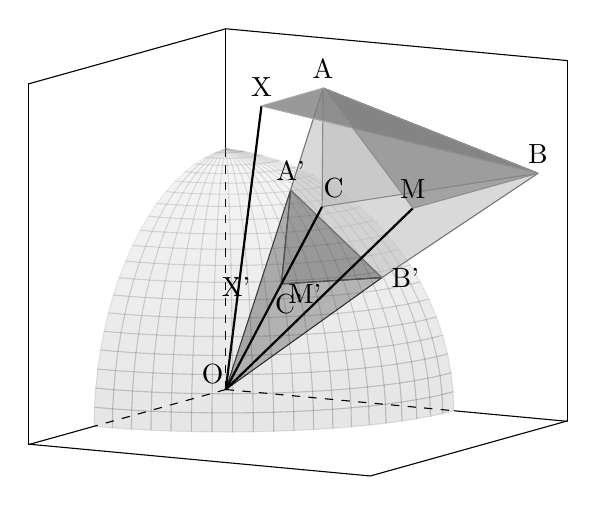
\begin{tikzpicture}
\begin{axis}[axis line style=white,view={120}{10},xmin=0,xmax=1.5,ymin=0,ymax=1.5,zmin=0,zmax=1.5,colormap/blackwhite,ticks=none]
\addplot3[color=black,thick] coordinates {(0,0,1.5) (0,1.5,1.5)};
\addplot3[color=black,thick] coordinates {(0,0,1.5) (1.5,0,1.5)};
\addplot3[color=black,thick] coordinates {(0,1.5,0) (0,1.5,1.5)};
\addplot3[color=black,thick] coordinates {(0,1.5,0) (1.5,1.5,0)};
\addplot3[color=black,thick] coordinates {(1.5,0,0) (1.5,0,1.5)};
\addplot3[color=black,thick] coordinates {(1.5,0,0) (1.5,1.5,0)};
\addplot3[color=black,dashed] coordinates {(0,0,0) (0,0,1)};
\addplot3[color=black,dashed] coordinates {(0,0,0) (0,1,0)};
\addplot3[color=black,dashed] coordinates {(0,0,0) (1,0,0)};
\addplot3[color=black] coordinates {(0,0,1) (0,0,1.5)};
\addplot3[color=black] coordinates {(0,1,0) (0,1.5,0)};
\addplot3[color=black] coordinates {(1,0,0) (1.5,0,0)};
\addplot3[patch,patch type=triangle,color=gray,fill opacity=0.6] coordinates {(0.0,0.0,0.0) (0.5774,0.5774,0.5774) (0.2,0.4,0.8944)
};
\addplot3[patch,patch type=triangle,color=gray,fill opacity=0.5] coordinates {(0.0,0.0,0.0) (0.5774,0.5774,0.5774) (0.2,0.8,0.5657)
};
\addplot3[patch,patch type=triangle,color=darkgray,fill opacity=0.5] coordinates {(0.5774,0.5774,0.5774) (0.2,0.4,0.8944) (0.2,0.8,0.5657)
};
\addplot3 [color=black,thick] coordinates {(0,0,0) (0.5774,0.5774,0.5774)};
\addplot3 [color=black,thick] coordinates {(0,0,0) (0.7309,0.4678,0.4970)};
\addplot3 [color=black,thick] coordinates {(0,0,0) (0.5709,0.6766,0.4651)};
\addplot3[opacity = 0.1,surf,z buffer = sort,samples = 21,variable = \u,variable y = \v,domain = 0:90,y domain = 0:90,]
    ({1*cos(u)*sin(v)}, {1*sin(u)*sin(v)}, {1*cos(v)});
\addplot3 [patch,patch type=rectangle,color=lightgray,fill opacity=0.6] coordinates{(0.2,0.4,0.8944) (0.3,0.6,1.35) (0.4,1.6,1.1) (0.2,0.8,0.5657)
};
\addplot3 [color=black,thick] coordinates {(0.5774,0.5774,0.5774) (1.0,1.0,1.0)};
\addplot3 [color=black,thick] coordinates {(0.7309,0.4678,0.4970) (2.5,1.6,1.7)};
\addplot3 [color=black,thick] coordinates {(0.5709,0.6766,0.4651) (1.35,1.6,1.1)};
\addplot3 [patch,patch type=triangle,color=lightgray,fill opacity=0.6] coordinates{(0.3,0.6,1.35) (1.0,1.0,1.0) (0.4,1.6,1.1)};
\addplot3 [patch,patch type=triangle,color=gray,fill opacity=0.8] coordinates{(0.3,0.6,1.35) (2.5,1.6,1.7) (0.4,1.6,1.1)};
\addplot3 [patch,patch type=triangle,color=gray,fill opacity=0.6] coordinates{(0.3,0.6,1.35) (1.35,1.6,1.1) (0.4,1.6,1.1)};
\node [anchor=south] at (axis cs: 0.1,0.0,0.0) {O};
\node [anchor=south] at (axis cs: 0.3,0.6,1.35) {A};
\node [anchor=south] at (axis cs: 0.4,1.6,1.1) {B};
\node [anchor=south] at (axis cs: 0.2,0.4,0.8944) {A'};
\node [anchor=west] at (axis cs: 0.2,0.8,0.5657) {B'};
\node [anchor=north] at (axis cs: 0.5774,0.61,0.5774) {C'};
\node [anchor=south] at (axis cs: 1.0,1.05,1.0) {C};
\node [anchor=south] at (axis cs: 0.7309,0.4678,0.4970) {X'};
\node [anchor=south] at (axis cs: 2.5,1.6,1.7) {X};
\node [anchor=south] at (axis cs: 0.5709,0.6766,0.4651) {M'};
\node [anchor=south] at (axis cs: 1.35,1.6,1.1) {M};
\end{axis}
\end{tikzpicture}
\caption{The geometric features of a subspace contextually projected based on an analysis of two input word-vectors.}
\label{fig:geofull}
\end{figure}
\fi

Figure~\ref{fig:geofull} illustrates a generic three dimensional subspace, with point $O$ as the origin.  Points $A$ and $B$ are the two word-vectors that have been used to select the dimensions which define this subspace, and are likewise the word-vectors which will be analysed through the geometry of the subspace.  In addition to these two points explicitly defined in terms of the values of projected word-vectors, two points are established based on an overall analysis of the dimensionality of the subspace: the \emph{mean point} $M$ and the \emph{maximal point} $X$.  $M$ is defined as the vector of all the mean values for all the dimensions $J$ delineating the subspace, so, if the dimensionality of $J$ is $d$, M can be defined formally as follows:

\begin{equation}
M = \{\mu(J_{1}),\ \mu(J_{2})...\ \mu(J_{d})\}
\end{equation}

\noindent And likewise, $X$ can be expressed in terms of an equation:

\begin{equation}
X = \{max(J_{1}),\ max(J_{2})...\ max(J_{d})\}
\end{equation}

\noindent Finally, a generic central point $C$, a vector with all dimensions set to the same value, is defined.  The universal value chosen to define the dimensions of this vector is the mean value of the mean point $M$, so, formally, this point is the vector of that mean value repeated $d$ times:

\begin{equation}
C = \{\mu(M),\ \mu(M)... \mu(M)\}
\end{equation}

\noindent In the analysis of the semantic relationship between $A$ and $B$ in a given projection, these three vectors will be used as anchor points to establish the situation of $A$ and $B$ relative to the subspace overall: where $C$ is an objectively central point in the subspace, $M$ is in a sense central to a subspace relative to its particular dimensional constitution, and $X$ is similarly indicative of the outermost possible extent of a particular subspace.  The underlying point here is that, due to the frequentist components of the information theoretic co-occurrence statistics used to build the base space described here, different dimensions have different distributional profiles.  To demonstrate this point, Table~\ref{tab:profiles} presents the mean values and standard deviations for the distribution of mean and maximum points from the top 20,000\footnote{less frequent dimensions tend to have higher PMI values overall, and also tend to be products of co-occurrences observed in quite obscure passages of the base corpus---it's worth recalling that a little more than half of the co-occurrence dimensions are observed only once.} most frequent co-occurrence dimensions, as well as the top five and bottom five values for each of these statistics for illustrative purposes.

\begin{table}
\centering
\begin{tabular}{lr|r}
\hline
& \multicolumn{1}{c}{\textsc{mean}} & \multicolumn{1}{c}{\textsc{max}} \\
\hline
\parbox[t]{2mm}{\multirow{5}{*}{\rotatebox[origin=c]{90}{\textsc{top}}}} & \emph{sofla:} 6.984 & \emph{nico:} 15.690 \\
& \emph{olya:} 6.326 & \emph{yeah:} 15.610 \\
& \emph{non-families:} 6.035 & \emph{superfamily:} 15.598 \\
& \emph{gmina:} 5.364 & \emph{eel:} 15.483 \\
& \emph{crambidae:} 5.485 & \emph{kermanshah:} 15.455 \\
\hline
\parbox[t]{2mm}{\multirow{5}{*}{\rotatebox[origin=c]{90}{\textsc{bottom}}}} & \emph{it:} 0.748 & \emph{he:} 3.903 \\
& \emph{they:} 0.812 & \emph{in:} 3.449 \\
& \emph{you:} 0.804 & \emph{of:} 3.379 \\
& \emph{this:} 0.789 & \emph{to:} 3.120 \\
& \emph{he:} 0.719 & \emph{and:} 2.993 \\
\hline
mean & 2.312 & 11.066 \\
std & 0.396 & 1.607 \\
\hline
\end{tabular}
\caption{Dimensional profiles in terms of mean and maximum PMI values along dimensions, including mean values and standard deviation as well as the top five and bottom five dimensions for each statistic.}
\label{tab:profiles}
\end{table}

The co-occurrence dimensions that tend to have lower mean and maximum values are clearly quite frequent words, and this is to be expected, given that the high frequency of independent observations of the word will drive PMI scores down for that word across the board.  The emergence of relatively infrequent words at the top end of the spectrum is then also to be expected.  The main point to note here, though, is that there is a broad range of possible mean and maximum values for a given dimension, and so the points $M$ and $X$ might be expected to vary considerably from subspace to subspace.  Moreover, this variance may in turn correspond to semantic features of a given subspace: it may be the case that a given type of relationship between input terms -- terms which are similar or dissimilar, literal or figurative in relationship to one another -- select for a subspace which has a particular orientation in terms of its dimensional profile.  More specific conjectures and results will be presented throughout the next two chapters.

In addition to the situation of the points $A$, $B$, $C$, $M$, and $X$ in a subspace, a normalised version of the subspace is considered, in which each vector is effectively measured at its intersection with a hypersphere of radius 1 emanating from the origin.  These points are represented as $A'$, $B'$, $C'$, $M'$, and $X'$ respectively in Figure~\ref{fig:geofull}.  The purpose of considering these points is to take measure of the way in which the various vectors in a given subspace relate to the subspace as a whole, regardless of the extent of these vectors.  So, for instance, the vectors $A$ and $B$ might have very different norms, but the angle $\angle AOB$ might still be very small---and, even then, the angle $\angle A'C'B'$ might be very large, suggesting that $A$ and $B$ both pass through the central region of the subspace but on different sides of the generic central point of the subspace.  One of the objectives of this analytical method is to test whether this kind of information, which can be captured through a robust geometric description of a subspace, is semantically indicative.

So finally the various geometric features available for the analysis of a subspace are systematically outlined in Table~\ref{tab:features}.  The points to be found in the space are broken down into three types, names, the word-vectors themselves (points $A$ and $B$), the generic points that emerge from an analysis of a subspace (points $C$, $M$, and $X$), and the normalised versions of all these points (for instance, $A'$).  The relationships between these points are construed across five categories as follows:

\begin{description}
\item[Distances] Euclidean distances, such as the distance between the two word-vectors $A$ and $B$ as well as the norms of the generic points, and, additionally, the mean distance of $A$ and $B$ from the origin;
\item[Angles] The angles at the vertexes of the generic points of a subspace, so for instance $\angle ACB$ formed by lines $\overline{AC}$ and $\overline{BC}$, as well as the normalised versions of these angles, and also the angles formed between the vectors of the generic points such as $\angle COM$;
\item[Means] The average distances from the word-vectors to generic points, as well as the average distances of the normalised versions of these points;
\item[Ratios] The ratio of the distances from the word-vectors to generic points, taking the lower of the two distances as the denominator, as well as the normalised version of the same measures;
\item [Fractions] The ratio of the mean distance from the origin of $A$ and $B$ to each of the three generic points, as well as the ratios of the generic points to one another.
\end{description}

\begin{table}
\centering
\begin{tabular}{ll}
\hline
\multicolumn{2}{c}{\textsc{distances}} \\
word-vectors & $\overline{AB}$ \\
generic points & $C$, \quad $M$, \quad $X$ \\
\hline
\multicolumn{2}{c}{\textsc{angles}} \\
word-vectors & $\angle AOB$, \quad $\angle ACB$, \quad $\angle AMB$, \quad $\angle AXB$ \\
normalised & $\angle A'C'B'$, \quad $\angle A'M'B'$, \quad $\angle A'X'B'$ \\
generic points & $\angle COM$, \quad $\angle COX$, \quad $\angle MOX$ \\
\hline
\multicolumn{2}{c}{\textsc{means}} \\
word-vectors & $\mu (A,B)$, \quad $\mu (\overline{AC},\overline{BC})$, \quad $\mu (\overline{AM},\overline{BM})$, \quad $\mu (\overline{AX},\overline{BX})$ \\
normalised & $\mu (\overline{A'C'},\overline{B'C'})$, \quad $\mu (\overline{A'M'},\overline{B'M'})$, \quad $\mu (\overline{A'X'},\overline{B'X'})$ \\
\hline
\multicolumn{2}{c}{\textsc{ratios}} \\
word-vectors & $A:B$, \quad $\overline{AC}:\overline{BC}$, \quad $\overline{AM}:\overline{BM}$, \quad $\overline{AX}:\overline{BX}$ \\
normalised & $\overline{A'C'}:\overline{B'C'}$, \quad $\overline{A'M'}:\overline{B'M'}$, \quad $\overline{A'X'}:\overline{B'X'}$ \\
\hline
\multicolumn{2}{c}{\textsc{fractions}} \\
word-vectors & $\mu (A,B)/C$, \quad $\mu (A,B)/M$, \quad $\mu (A,B)/X$ \\
generic points & $C/M$, \quad $C/X$, \quad $M/X$ \\
\hline
\end{tabular}
\caption{Geometric features extrapolated from a subspace projected based on an analysis of two two input terms $A$ and $B$.}
\label{tab:features}
\end{table}

\noindent These features have been selected as indicative of the overall comportment of the subspaces from which they are extracted, and, both independently and in conjunction, are expected to serve as indicators of the semantic phenomena characteristic of the word-vectors used to generate the subspace into which they are projected.  So, for instance, I will predict (incorrectly, it turns out) that the distance $\overline{AB}$ will be one of the strongest indicators of semantic relatedness.  Furthermore, the extrapolation of the generic features of a subspace is expected to indicate more general patterns of co-occurrence that are associated with semantic phenomena such as similarity and metaphor.  When lower frequency dimensions are jointly selected by a pair of words, a (more correction) expectation will be that this indicates a high degree of conceptual overlap between the words' referrents, and therefore a high degree os similarity.

As a more general hypothesis, I surmise that different sets of geometric features will collectively be predictive of different semantic phenomena.  One of the primary objectives of the empirical work described in the next two chapters will be to establish a methodology for mapping features to phenomena and then using these correspondences as a mechanism for understanding the statistical characteristics that allow for the computational extraction of semantically and contextually useful information from large scale corpora.  It will therefore ultimately be the comparison of the groupings of features corresponding to specific semantic that will provide the most significant outputs of the research reported here, and so the arrangement of features in terms of types and categories as outlined in Table~\ref{tab:features} is in this regard a schematic for the computational experimentation and corresponding evaluation and analysis at the core of this thesis.

This more or less sets the stage for the empirical section of the thesis.  The only outstanding issue is the establishment of the models which will serve as points of comparison for my methodology.

\section{Comparing to Alternative Approaches}
In order to evaluate the effectiveness of my methodology, it will naturally be necessary to compare the preformance of the models I develop against other models.  One way of doing this will, of course, be to compare to results other researchers have obtained experimenting with the data which will serve as the foundation for the empirical results reported in the next two chapters.  In the cases of results reported by other researchers, though, similar but variously different corpora have been used to train other models described in the literature.  This is to be expected, and the results for large scale corpora should be fairly generalisable assuming a sensible choice of data (and the use of Wikipedia as all or a large portion of base data is quite common in the field), but nonetheless it will be useful to establish a baseline of results generated using models trained on the exact same data towards which I apply my methdology.  In the cases of metaphor and semantic type coercion in particular, which will be examined in Chapter~\ref{chap:figurative}, the datasets explored are relatively new and have not been approached by many researchers in the field, so any additional point of comparison will be valuable in evaluating my methodology.

Moreover, in most cases, other models have been designed in a task specific way: so, for instance, \cite{SchwartzEA2015} have developed a syntactic heuristic for identifying semantic similarity as compared to relatedness in particular, and \cite{GutierrezEA2016} develop a model that generates compositional adjective-noun representations geared towards metaphor detection.  One of the key features of my models is that they are intended to be \emph{general}: the geometries generated by my methodology are expected to be replete with semantic interpretability, allowing for the same potential for diverse and often surprising conceptualisation corresponding to the infinitely combinatory characteristic of natural language in use.  For this reason, it is desirable to have a base case of a generic model that can be compared across the board to all the different tasks handled by my methodology.

With all this in mind, I propose two different points of comparison that, in addition to results extracted from existing literature, will be applicable to all subsequent experiments described here.  The first is actually a pair of techniques for interpretting my base space in a non-contextual way, and so will serve as a way of measuring the degree to which building context specific subspaces enhances the ability to model semantic phenomena.  The second is an application of a well known and highly productive neural network model to the same underlying data that I've used.  This will serve as a mechanism for comparing my results to what has proved to be another very effective methodology for the statistical modelling of semantics in general.

\subsection{Static Interpretations of the Base Space}
In cases where the geometry being explored involves just target word-vectors and generic points of a space -- so, for all the features described in Table~\ref{tab:features} -- it is computationally tractable to treat the sparse base matrix from which subspaces are projected as a semantically interpretable space in its own right.  This is because universal generic points (the mean point for all dimensions, the maximum point for all dimensions, and the central point based on the average value of the mean point) can be discovered through a one-off caluculation, and the word-vectors themselves will be relatively sparse.  In the most honerous case of comparing two orthogonal word-vectors using the \textsc{indy} technique, the total number of scalars involved in the computations of geometric features would be the sum of the number of non-zero dimensions for each word-vector, so something on the order of thousands to tens of thousands of values---not that bad, computationally speaking.

Of course, the norms of the generic points in such a general space will be extremely high compared to any given actual word-vector, since these generic points will have non-zero values in several million dimensions.  With this in mind, a second and more typical approach to building a general and computable distributional semantic space out of my base space of co-occurrence statistics is to through matrix factorisation: using singular value decomposition, I project the base space onto the top most informational eigenvectors up to a dimensionality to match the parameters tested using my context specific dimensional selection techniques.\footnote{In practice, the \texttt{sklearn} python module's PCA method is used to do this.}  Because of computability constraints, I take the top 100 to 50,000 most frequent word types as the vocabulary for this model, and consider the top 10,000 most frequent co-occurrence terms as the dimensions of the matrix to be factorised.  This means that 1,979 of the 1,998 word tokens in the SimLex999 dataset \citep[][discussed in detail in Chapter~\ref{chap:concepts}]{HillEA2014} are included in the vocabulary, and 

of the co-occurrence events tabulated in the base space are represented in the decomposed model.

Because SVD produces a space with a barycenter at the origin, the factorised model is not suitable for generating the generic points which are key features of my contextual models.  In order to m

barycentre 

\subsection{A Model Trained Using a Neural Network}
In addition to the interpretations of the statistical base space described above, I also use the \texttt{word2vec} method
